\subsubsection*{\large Используемые структуры}
\begin{lstlisting}[caption=Структура open\_flags]
struct open_flags {
	int open_flag;
	umode_t mode;
	int acc_mode;
	int intent;
	int lookup_flags;
};
\end{lstlisting}

\begin{lstlisting}[caption=Структура filename]
struct filename {
	const char *name;
	const __user char *uptr;
	int refcnt;
	struct audit_names *aname;
	const char iname[];
};	
\end{lstlisting}

\begin{lstlisting}[caption=Структура nameidata]
struct nameidata {
	struct path path;
	struct qstr last;
	struct path root;
	struct inode *inode;
	unsigned int flags, state;
	unsigned seq, m_seq, r_seq;
	int last_type;
	unsigned depth;
	int total_link_count;
	struct saved {
		struct path link;
		struct delayed_call done;
		const char *name;
		unsigned seq;
	} *stack, internal[EMBEDDED_LEVELS];
	struct filename	*name;
	struct nameidata *saved;
	unsigned root_seq;
	int dfd;
	kuid_t dir_uid;
	umode_t dir_mode;
};	
\end{lstlisting}



\section*{Схемы алгоритмов}

\begin{figure}[ht!]
	\centering
	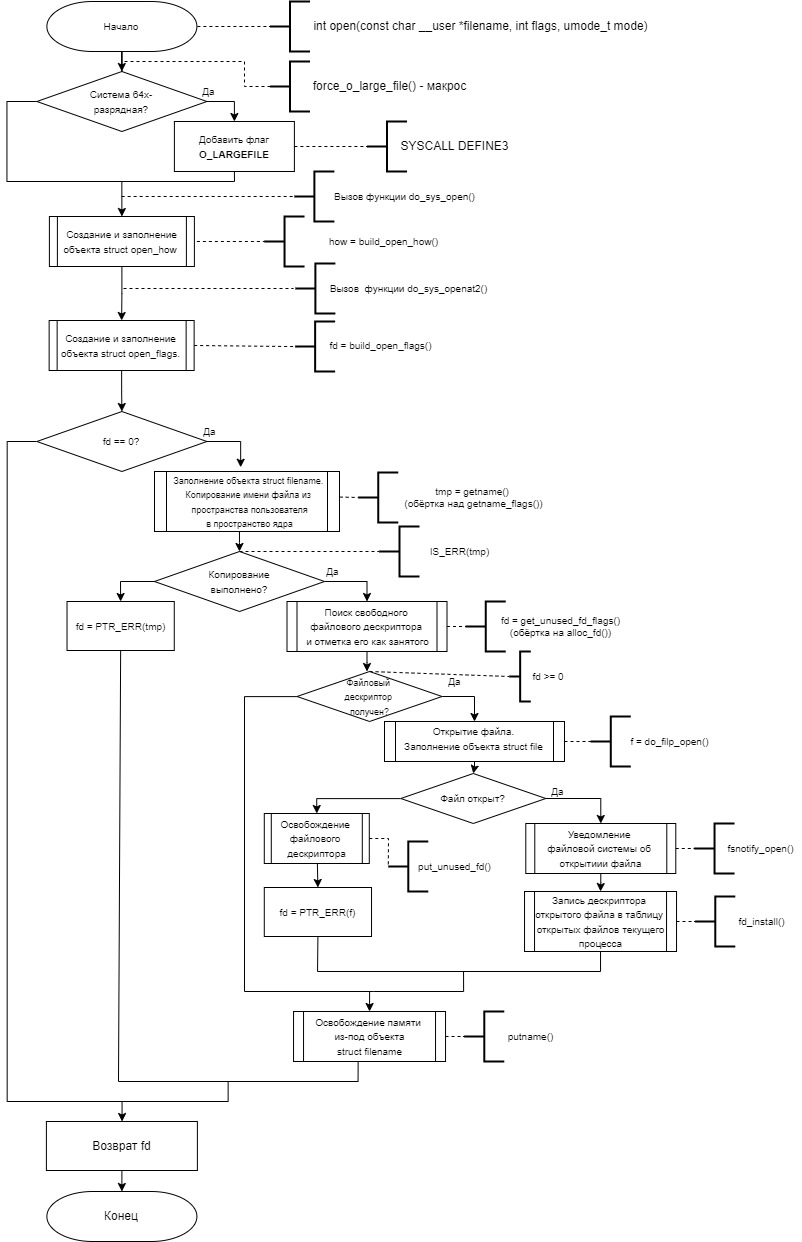
\includegraphics[scale=0.5]{open}
	\caption{Схема алгоритма работы системного вызова open()}
\end{figure}

\pagebreak

\begin{figure}[ht!]
	\centering
	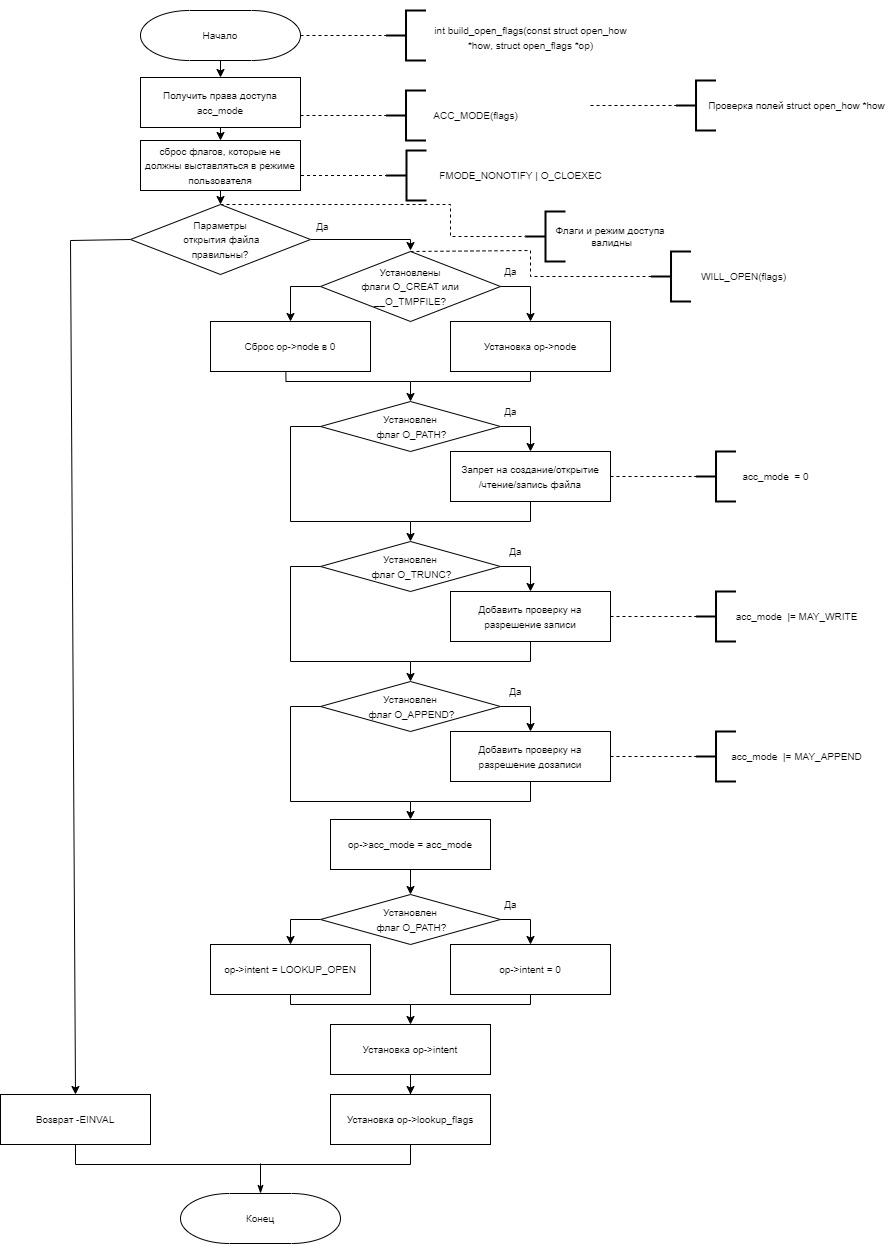
\includegraphics[scale=0.55]{build_open_flags}
	\caption{Схема алгоритма работы функции build\_open\_flags()}
\end{figure}

\pagebreak

\begin{figure}[ht!]
	\centering
	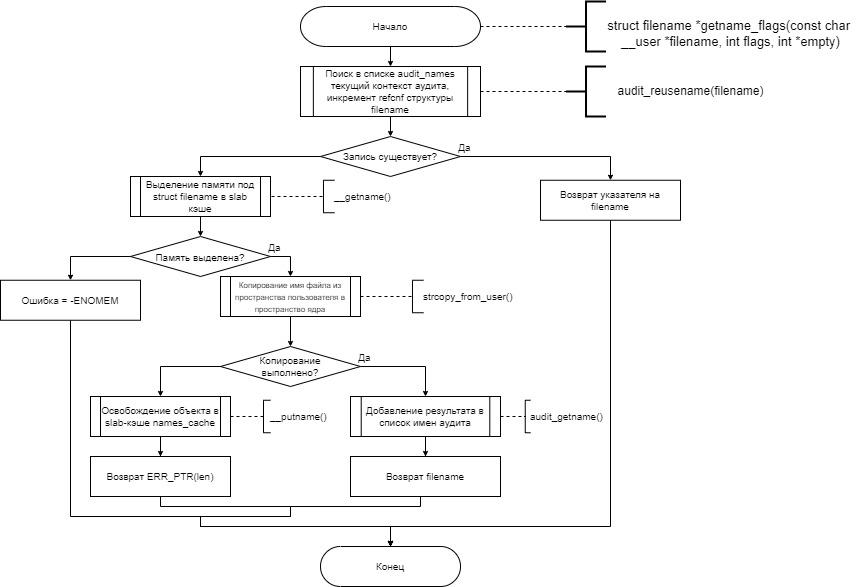
\includegraphics[scale=0.55]{getname_flags}
	\caption{Схема алгоритма работы функции getname\_flags()}
\end{figure}

\pagebreak

\begin{figure}[ht!]
	\centering
	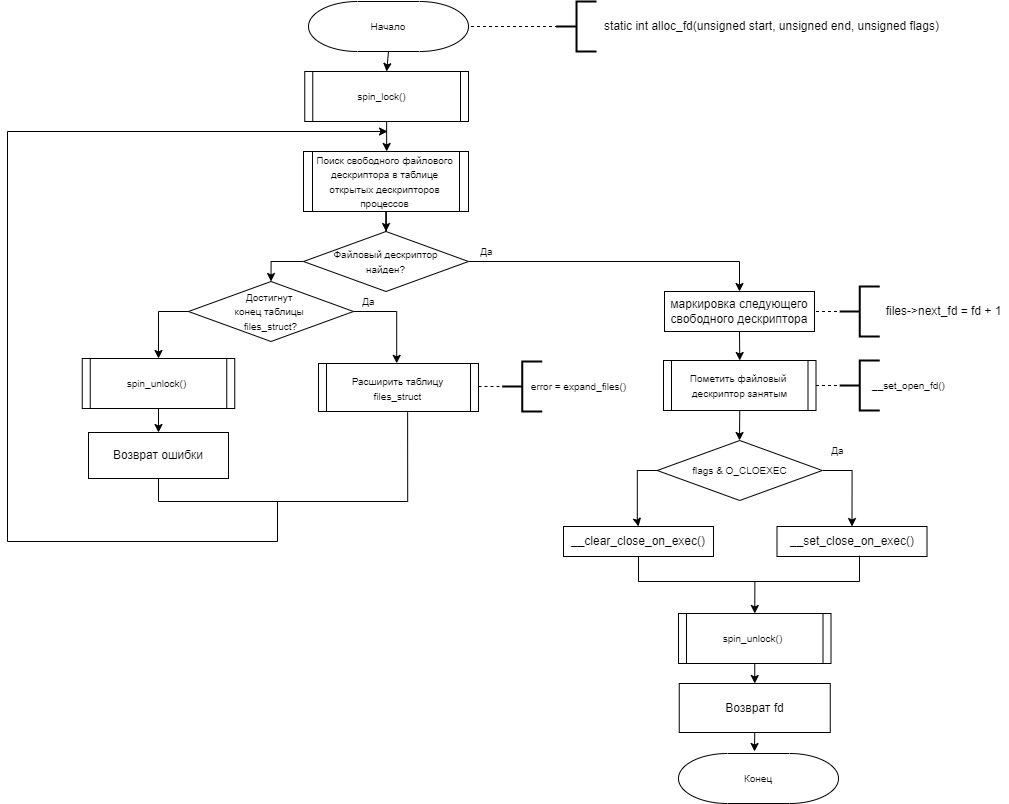
\includegraphics[scale=0.47]{alloc_fd}
	\caption{Схема алгоритма работы функции alloc\_fd()}
\end{figure}

\pagebreak

\begin{figure}[ht!]
	\centering
	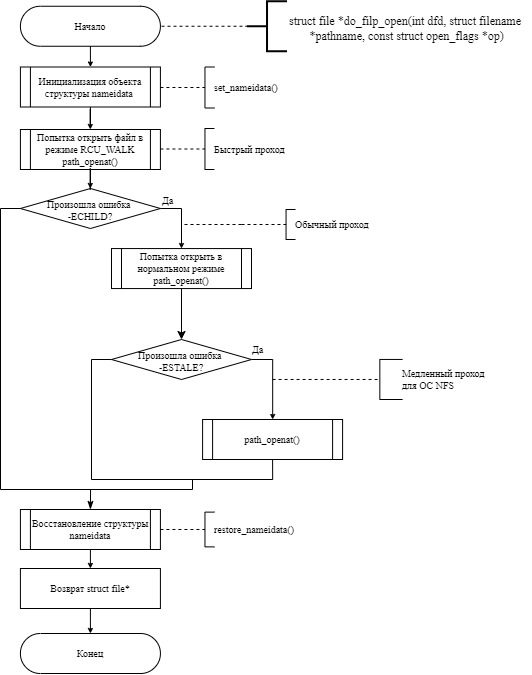
\includegraphics[scale=0.6]{do_filp_open}
	\caption{Схема алгоритма работы функции do\_filp\_open()}
\end{figure}

\pagebreak

\begin{figure}[ht!]
	\centering
	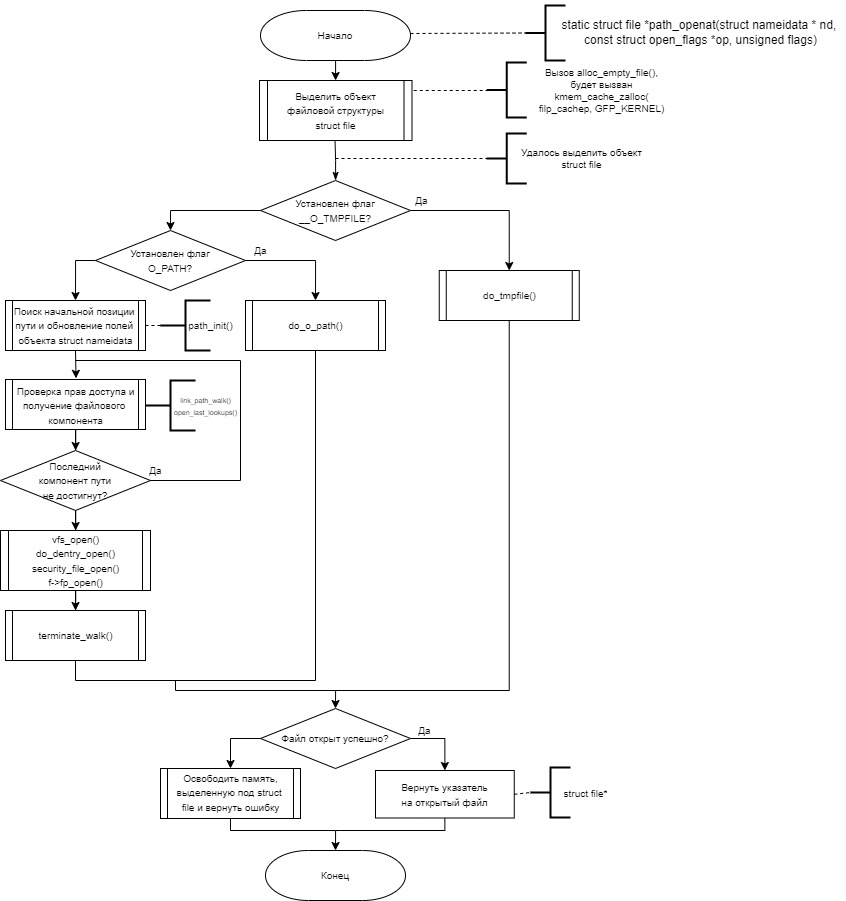
\includegraphics[scale=0.6]{path_openat}
	\caption{Схема алгоритма работы функции path\_openat()}
\end{figure}

\pagebreak

\begin{figure}[ht!]
	\centering
	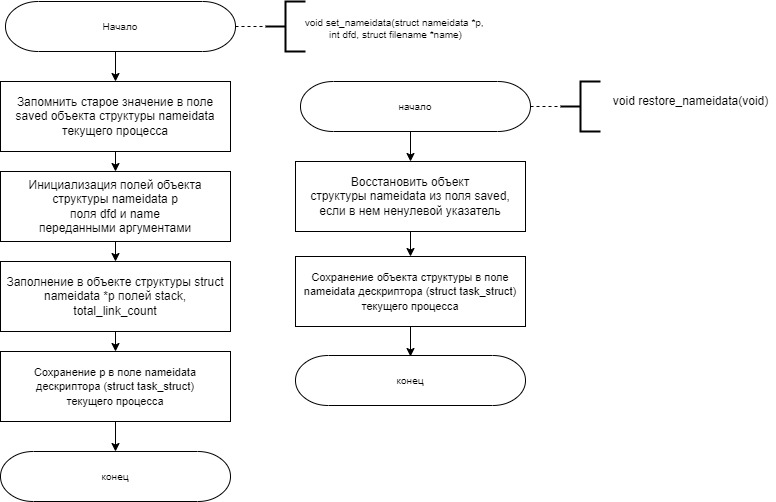
\includegraphics[scale=0.6]{set_restore_nameidata}
	\caption{Схема алгоритма работы функций set\_nameidata() и restore\_nameidata()}
\end{figure}


LOOKUP\_RCU --- флаг для открытия файла в режиме RCU\_walk (Допускает
возможность одновременного доступа).

LOOKUP\_REVAL --- флаг для ФС NFS O\_APPEND.

O\_APPEND может проводить к потери данных файлов в ФС NFS,
если одновременно добавл. данные нескольких процессов.
Нельзя избежать ускорение гонки.

NFS не поддерживает добавление в файл, потому клиентское ядро имитирует такое поведение.

\pagebreak



\begin{figure}[ht!]
	\centering
	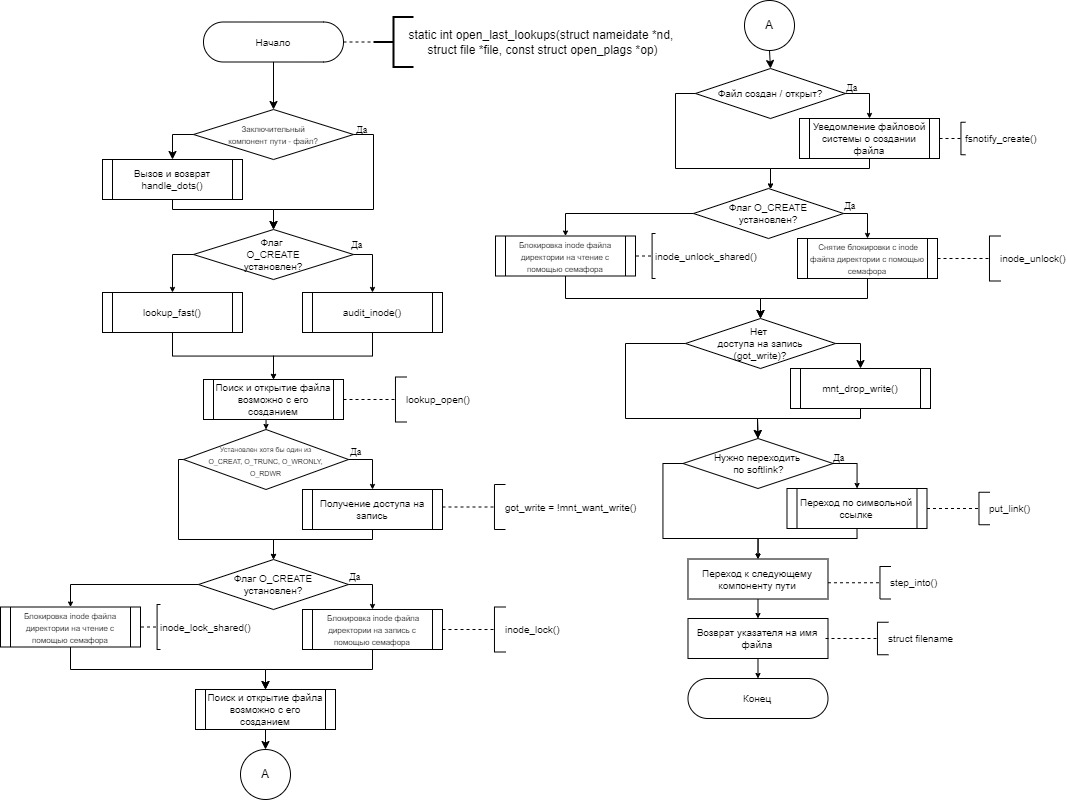
\includegraphics[scale=0.47]{open_last_lookups}
	\caption{Схема алгоритма работы функции open\_last\_lookups()}
\end{figure}


\begin{figure}[ht!]
	\centering
	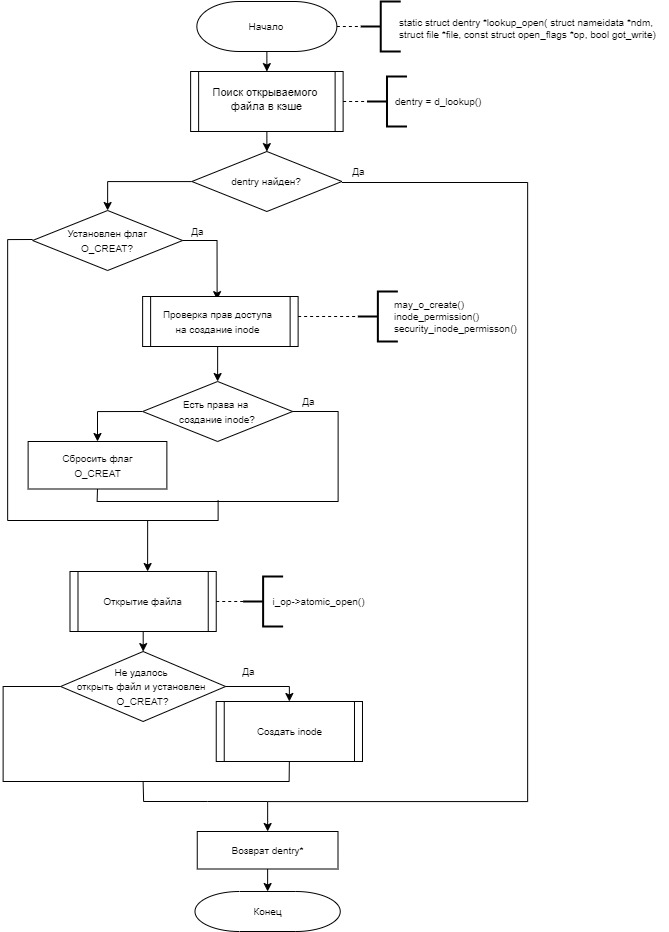
\includegraphics[scale=0.6]{lookup_open}
	\caption{Схема алгоритма работы функции lookup\_open()}
\end{figure}

\begin{figure}[ht!]
	\centering
	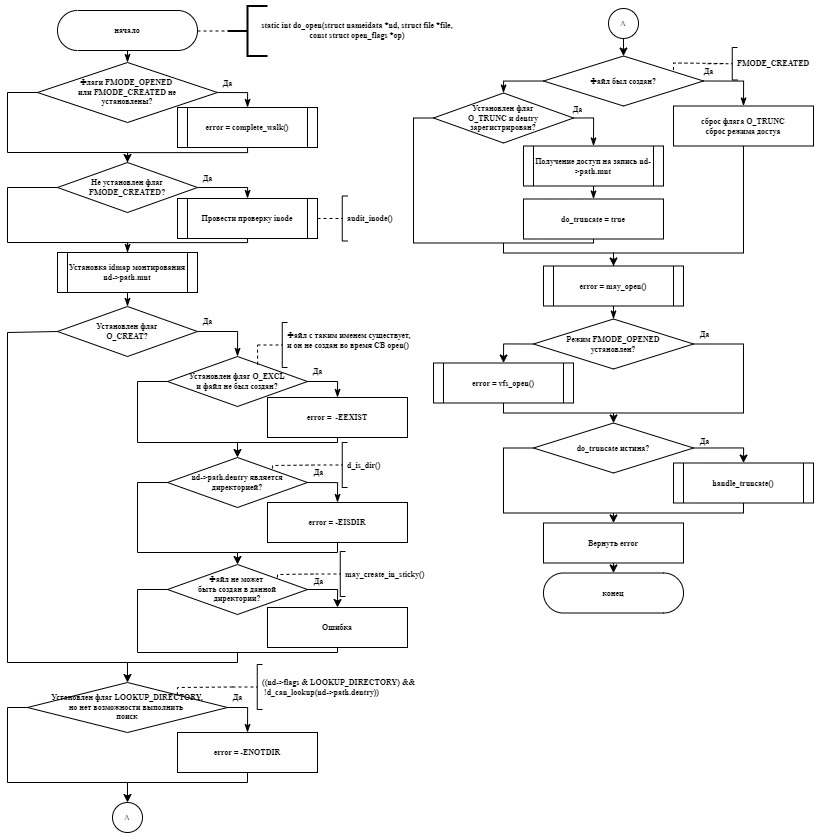
\includegraphics[scale=0.6]{do_open}
	\caption{Схема алгоритма работы функции do\_open()}
\end{figure}

